\subsection{Problem 3: Surat dari Tetangga}

\subsubsection{Identifikasi Masalah}

Pada Milestone 1, sistem dibangun di atas dua asumsi sederhana. Perubahan data dari sumber dianggap hanya menambah kolom opsional (\textit{additive}), sedangkan jalur akses klien hanya bersifat baca (\textit{read-only}). Pada Milestone 2, kedua asumsi tersebut tidak lagi memadai karena muncul empat persoalan utama:

\begin{enumerate}
  \item \textbf{Perubahan skema yang merusak kontrak data dan tercampurnya jenis kegagalan (Kriteria 1 dan 2).}
  Sumber seperti PVMBG dapat mengubah struktur data tanpa koordinasi, misalnya mengganti nama atau tipe kolom wajib hingga menghapusnya. Di Milestone 1, Aggregator hanya menulis peringatan log lalu membuang data tersebut sehingga informasi bencana hilang. Sistem juga belum membedakan gangguan sementara dari kegagalan permanen. Dalam literatur, hal ini mencakup \textbf{\textit{backward-incompatible schema drift}}, pola karantina (\textbf{\textit{dead letter queue / quarantine}}), dan pemisahan \textit{transient failure} versus \textit{permanent failure}.

  \item \textbf{Masukan rusak atau berukuran ekstrem yang menjatuhkan layanan (Kriteria 3).}
  Sumber eksternal dapat mengirim JSON terpotong, struktur bersarang sangat dalam, deretan byte UTF-8 rusak, atau ukuran \textit{payload} terlalu besar. Memanggil \texttt{JSON.parse} langsung dapat memicu \textit{stack overflow} atau kehabisan memori di kontainer \texttt{512Mi} lalu menjatuhkan \textit{pod}. Satu pesan cacat pun bisa melumpuhkan data sumber lain yang sehat. Gangguan ini dikenal sebagai \textbf{\textit{poison pill input}}, yang diatasi melalui \textbf{\textit{bounded parsing}} dan \textbf{\textit{fault isolation}}.

  \item \textbf{Pemrosesan ulang yang berisiko merusak data dan akses yang terlalu longgar (Kriteria 4 dan 5).}
  Isi pesan gagal berisiko membocorkan rincian galat internal sehingga hanya \textbf{BNPB Internal Ops} yang berhak memeriksa dan memicu pemrosesan ulang (\textit{replay}). Memproses ulang pesan secara paralel tanpa aturan urutan berisiko membuat data lama menimpa keadaan terbaru atau menciptakan dokumen ganda. Literatur merujuk hal ini pada \textbf{\textit{authorized replay}}, \textbf{\textit{idempotent write}}, \textbf{\textit{per-key ordering}}, \textbf{\textit{optimistic version guard}}, dan \textbf{\textit{server-side RBAC}}.

  \item \textbf{Kehilangan atau duplikasi laporan Tim Lapangan saat hilir terganggu (Kriteria 6).}
  Tim Lapangan mengirim laporan lewat \path{POST /field-reports} dengan koneksi terbatas, sementara \textit{broker} RabbitMQ atau \textit{consumer} hilir dapat melambat atau mati. Jika API langsung membalas \texttt{202 Accepted} lalu menulis terpisah ke basis data dan \textit{broker}, kegagalan di tengah proses akan menghilangkan laporan atau menggandakannya. Persoalan klasik ini disebut \textbf{\textit{dual-write problem}} pada pola \textit{asynchronous request-reply}, yang diselesaikan melalui \textbf{\textit{transactional outbox pattern}}, pengiriman minimal sekali, serta \textit{idempotent consumer}.
\end{enumerate}

\subsubsection{Rancangan Solusi dan Mekanisme yang Dipilih}

Rancangan Problem 3 memisahkan tahap penyimpanan data mentah ke media persisten dari tahap validasi skema dan distribusi ke layanan hilir. Dengan pemisahan ini, data tidak akan hilang meski gagal diparse atau meski \textit{broker} sedang mati. Alur lengkapnya diperlihatkan pada \textbf{Gambar~\ref{fig:p3-arch}}.

\begin{figure}[H]
  \centering
  \IfFileExists{figures/p3-arsitektur-skema-outbox.png}{%
    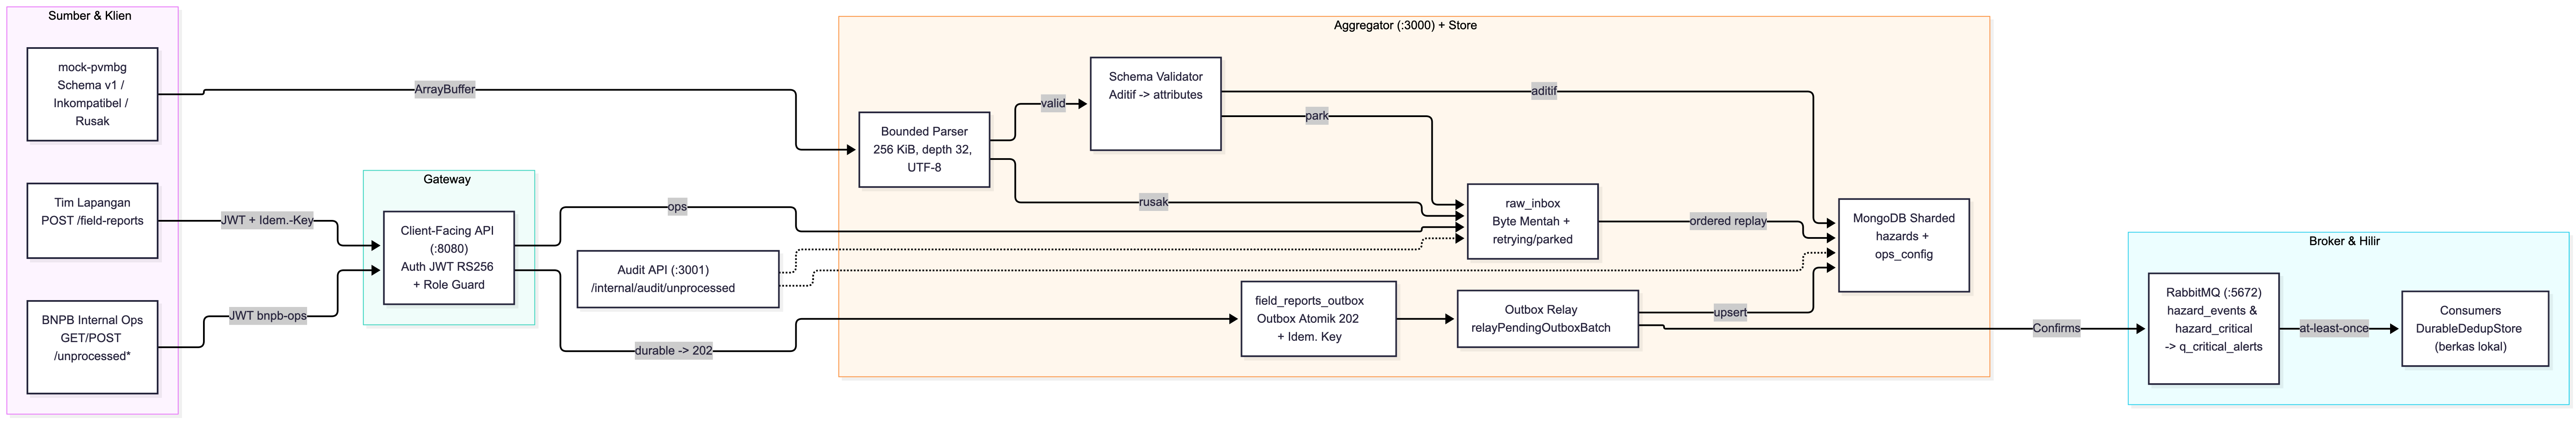
\includegraphics[width=0.95\linewidth]{p3-arsitektur-skema-outbox.png}%
  }{%
  \resizebox{\linewidth}{!}{%
  \begin{tikzpicture}[
    every node/.style={font=\sffamily\footnotesize},
    box/.style={draw=black!65, rounded corners=3pt, fill=white, align=center, inner sep=5pt, minimum width=3.1cm, minimum height=0.95cm},
    store/.style={draw=blue!55!black, rounded corners=2pt, fill=blue!6, align=center, inner sep=5pt, minimum width=3.2cm, minimum height=0.95cm},
    group/.style={draw=black!35, dashed, rounded corners=4pt, fill=black!2, inner sep=10pt},
    arr/.style={-{Stealth[length=2.2mm]}, thick, draw=black!75},
    lbl/.style={font=\sffamily\scriptsize, fill=white, inner sep=1.5pt, align=center}
  ]
    % Kolom 1: Sumber & Klien (x = 0)
    \node[box] (pvmbg) at (0, 4.8) {\textbf{mock-pvmbg}\\{\scriptsize Schema v1 / Inkompatibel / Rusak}};
    \node[box] (ops)   at (0, 2.0) {\textbf{BNPB Internal Ops}\\{\scriptsize GET/POST /unprocessed*}};
    \node[box] (ft)    at (0, 0.0) {\textbf{Tim Lapangan}\\{\scriptsize POST /field-reports}};

    % Kolom 2: Client-Facing API (x = 5.7)
    \node[box] (auth)  at (5.7, 1.0) {\textbf{Client-Facing API (:8080)}\\{\scriptsize Auth JWT RS256 + Role Guard}};

    % Kolom 3 & 4: Aggregator & Store (x = 12.6 dan 17.8)
    \node[box]   (bp)     at (12.6, 4.8) {\textbf{Bounded Parser}\\{\scriptsize 256 KiB, depth 32, UTF-8}};
    \node[box]   (val)    at (17.8, 4.8) {\textbf{Schema Validator}\\{\scriptsize Aditif $\to$ attributes}};
    \node[store] (inbox)  at (12.6, 2.4) {\textbf{raw\_inbox}\\{\scriptsize Byte Mentah + retrying/parked}};
    \node[store] (canon)  at (17.8, 2.4) {\textbf{MongoDB Sharded}\\{\scriptsize hazards + ops\_config}};
    \node[store] (outbox) at (12.6, 0.0) {\textbf{field\_reports\_outbox}\\{\scriptsize Outbox Atomik 202 + Idem. Key}};
    \node[box]   (relay)  at (17.8, 0.0) {\textbf{Outbox Relay}\\{\scriptsize relayPendingOutboxBatch}};

    % Kolom 5: Audit, Broker & Consumers (x = 23.4)
    \node[box] (audit) at (23.4, 4.8) {\textbf{Audit API (:3001)}\\{\scriptsize /internal/audit/unprocessed}};
    \node[box] (rmq)   at (23.4, 0.0) {\textbf{RabbitMQ (:5672)}\\{\scriptsize hazard\_events \& hazard\_critical}\\{\scriptsize $\to$ q\_critical\_alerts}};
    \node[box] (cons)  at (23.4, 2.4) {\textbf{Consumers}\\{\scriptsize DurableDedupStore (berkas lokal)}};

    % Grouping latar belakang
    \begin{scope}[on background layer]
      \node[group, fit=(pvmbg)(ops)(ft), label={[font=\sffamily\scriptsize\bfseries]above:Sumber \& Klien}] {};
      \node[group, fit=(auth), label={[font=\sffamily\scriptsize\bfseries]above:Gateway}] {};
      \node[group, fit=(bp)(val)(inbox)(canon)(outbox)(relay), label={[font=\sffamily\scriptsize\bfseries]above:Aggregator (:3000) + Store}] {};
      \node[group, fit=(rmq)(cons), label={[font=\sffamily\scriptsize\bfseries]below:Broker \& Hilir}] {};
    \end{scope}

    % Panah
    \draw[arr] (pvmbg) -- node[lbl, above] {ArrayBuffer} (bp);
    \draw[arr] (bp) -- node[lbl, above] {valid} (val);
    \draw[arr] (bp) -- node[lbl, left] {rusak} (inbox);
    \draw[arr] (val) -- node[lbl, right] {aditif} (canon);
    \draw[arr] (val.south west) -- node[lbl, above, sloped] {park} (inbox.north east);
    \draw[arr] (inbox) -- node[lbl, above] {ordered replay} (canon);

    \draw[arr] (ops.east) -- ++(1.1,0) node[lbl, above, midway] {JWT bnpb-ops} |- ([yshift=2mm]auth.west);
    \draw[arr] (ft.east)  -- ++(1.1,0) node[lbl, below, midway] {JWT + Idem.-Key} |- ([yshift=-2mm]auth.west);

    \draw[arr] ([yshift=2mm]auth.east)  -- ++(0.9,0) |- node[lbl, above, pos=0.76] {ops} (inbox.west);
    \draw[arr] ([yshift=-2mm]auth.east) -- ++(0.9,0) |- node[lbl, below, pos=0.76] {durable $\to$ 202} (outbox.west);

    \draw[arr] (outbox) -- (relay);
    \draw[arr] (relay) -- node[lbl, right] {upsert} (canon);
    \draw[arr] (relay) -- node[lbl, above] {Confirms} (rmq);
    \draw[arr] (rmq) -- node[lbl, right] {at-least-once} (cons);

    \draw[arr, dashed] ([yshift=-3mm]audit.west) -- ++(-0.9,0) |- ([yshift=2mm]canon.east);
    \draw[arr, dashed] (audit.north) -- ++(0,0.85) -| (inbox.north);
  \end{tikzpicture}%
  }%
  }
  \caption{Diagram Rancangan Solusi Problem 3}
  \label{fig:p3-arch}
\end{figure}

Rancangan ini diwujudkan melalui empat mekanisme utama berikut.

\paragraph*{1. Kebijakan Evolusi Skema dan Validator Adaptif (P3-K1)}
Batas antara perubahan yang diterima otomatis dan perubahan yang ditolak diatur dalam \texttt{validateAndMapPvmbgRecord} di \path{aggregator/src/p3/schemaValidator.ts}.

\begin{itemize}
  \item \textbf{Perubahan yang diterima otomatis:} sistem menerima penambahan kolom baru di luar skema kanonik, misalnya \texttt{confidence\_level}. Seluruh kolom tambahan tersebut ditampung ke dalam objek \texttt{attributes} pada \texttt{HazardEvent}. Dengan cara ini, Aggregator tidak perlu dimulai ulang dan struktur basis data tidak perlu dimigrasi.
  \item \textbf{Perubahan yang ditolak dan dikarantina:} sistem menolak perubahan yang merusak kontrak data wajib. Penolakan meliputi penggantian nama kolom wajib seperti \texttt{volcano\_id}, perubahan tipe angka menjadi teks pada \texttt{eruption\_count\_24h}, penghapusan kolom wajib, serta nilai \texttt{alert\_level} di luar daftar resmi \texttt{NORMAL}, \texttt{WASPADA}, \texttt{SIAGA}, atau \texttt{AWAS}.
\end{itemize}

Untuk keperluan pengujian terkontrol, simulator pada \path{mock-pvmbg/src/index.ts:132-238} memperluas \path{POST /admin/schema-version} agar mendukung seluruh mode perubahan skema. Simulator juga menyediakan \path{POST /admin/malformed} untuk memicu empat jenis \textit{payload} rusak.

\begin{lstlisting}
// aggregator/src/p3/schemaValidator.ts:80-103
if (typeof record['volcano_id'] !== 'string' || record['volcano_id'].trim() === '') {
    return { ok: false, reason: "schema_incompatible: missing or renamed required field 'volcano_id'", sourceRefId };
}
if (typeof record['alert_level'] !== 'string' || !VALID_ALERT_LEVELS.has(record['alert_level'].toUpperCase())) {
    return {
        ok: false,
        reason: `schema_incompatible: field 'alert_level' missing or invalid (${typeof record['alert_level']}: ${String(record['alert_level'])})`,
        sourceRefId,
    };
}
const eruptions = parseFiniteNumber(record['eruption_count_24h'], rules.coerceNumericStrings);
if (eruptions === null) {
    return {
        ok: false,
        reason: `schema_incompatible: field 'eruption_count_24h' must be number, got ${typeof record['eruption_count_24h']}`,
        sourceRefId,
    };
}
\end{lstlisting}

\paragraph*{2. \textit{Bounded Parser} dan Pengarsipan Byte Mentah (P3-K2, K3)}
Agar pesan rusak tidak menjatuhkan proses Node.js, Aggregator mengambil respons sebagai \textit{array} byte mentah (\path{aggregator/src/index.ts:255-268}). Data tersebut lalu divalidasi secara bertahap lewat fungsi \texttt{parseBoundedRawJson} pada \path{aggregator/src/p3/boundedJson.ts:14-85}.

\begin{enumerate}
  \item \textbf{Pemeriksaan batas ukuran:} setiap respons melebihi \texttt{MAX\_PAYLOAD\_BYTES} (\texttt{262.144 byte} atau \texttt{256 KiB}) langsung ditolak sebelum didekodekan.
  \item \textbf{Pemeriksaan UTF-8 ketat:} dekode memakai \texttt{TextDecoder('utf-8', \{ fatal: true \})} agar urutan byte cacat langsung terdeteksi tanpa berubah menjadi karakter pengganti.
  \item \textbf{Penghitungan kedalaman iteratif:} fungsi \texttt{measureJsonDepth} memindai kurung pembuka di luar \textit{string} dengan waktu linear. Jika kedalaman melebihi \texttt{MAX\_JSON\_DEPTH} (\texttt{32}), fungsi berhenti sebelum memanggil \texttt{JSON.parse}.
  \item \textbf{Penangkapan JSON terpotong:} panggilan \texttt{JSON.parse} dibungkus blok \texttt{try/catch} sehingga JSON terputus mencatat galat \texttt{malformed\_json} tanpa menjatuhkan proses.
\end{enumerate}

Pesan yang gagal disimpan utuh ke koleksi \texttt{raw\_inbox} menggunakan tipe BSON \texttt{Binary} (\path{MongoRawInbox.appendFailure}, \path{rawInbox.ts:172-215}). Dokumen dilengkapi \textit{hash} \texttt{raw\_sha256}, \texttt{source}, \texttt{reason}, waktu terima, serta salah satu status berikut.

\begin{itemize}
  \item \textbf{Status \texttt{retrying}:} dipakai untuk gangguan sementara seperti basis data yang sedang terputus. Pekerja latar belakang mengunci pesan secara atomik memakai \texttt{claim\_token} dan mencoba ulang menggunakan \textit{exponential backoff} ($1\text{ s} \cdot 2^{\text{attempt}-1}$, maks $30\text{ s}$) plus acakan \textit{jitter} $\pm 25\%$ hingga lima kali percobaan.
  \item \textbf{Status \texttt{parked}:} dipakai untuk kegagalan permanen seperti ketidaksesuaian skema atau masukan rusak. Pesan ini tidak dicoba ulang otomatis dan menunggu penyesuaian dari operator.
\end{itemize}

\paragraph*{3. Akses Khusus Internal Ops dan \textit{Ordered Replay} (P3-K4, K5)}
Pembatasan akses ditegakkan langsung di server oleh fungsi \texttt{ensureInternalOps} pada \path{client-api/src/routes/unprocessed.ts:7-16}.

\begin{lstlisting}
// client-api/src/routes/unprocessed.ts:7-16
function ensureInternalOps(res: import('express').Response): boolean {
    const clientId = String(res.locals.clientId ?? '');
    if (clientId !== 'bnpb-ops') {
        getLog(res).warn({ client_id: clientId }, 'non-ops access to failed messages denied');
        res.status(403).json({
            error: 'insufficient_scope',
            error_description: 'Failed messages may only be inspected or replayed by BNPB Internal Ops',
        });
        return false;
    }
    return true;
}
\end{lstlisting}

Permintaan tanpa token dibalas \textbf{HTTP 401}, sedangkan klien \texttt{media} dan \texttt{field-team} ditolak dengan \textbf{HTTP 403}. Hanya token milik \texttt{bnpb-ops} yang boleh memanggil \path{GET /unprocessed}, \path{POST /unprocessed/schema-rules}, dan \path{POST /unprocessed/replay}. Sementara itu, auditor membaca \path{raw\_inbox} lewat \path{GET /internal/audit/unprocessed} (\path{routes.ts:111-125}) memakai \texttt{\textless{}audit-token\textgreater{}}.

Setelah pembaruan aturan skema disinkronkan lintas replika via koleksi \texttt{ops\_config} (\path{aggregator/src/index.ts:85-105}), fungsi \texttt{execute\allowbreak Ordered\allowbreak Replay} (\path{rawInbox.ts:490-526}) menjalankan tiga pengaman berikut.

\begin{enumerate}
  \item \textbf{Penjagaan urutan per \texttt{source\_ref\_id}:} pesan diproses dari yang paling awal masuk. Jika satu pesan pada kunci tertentu masih gagal, kunci tersebut diblokir agar pesan baru tidak mendahuluinya (\texttt{hasBlockingFailure}).
  \item \textbf{Penulisan \textit{idempotent} dan penjaga versi:} penulisan memakai \texttt{hazard\_id} deterministik disertai \texttt{eventVersion} berbasis \texttt{occurred\_at} sehingga pemrosesan ulang tidak menimbulkan duplikasi atau menimpa data terbaru.
  \item \textbf{Pembatasan laju:} kecepatan pemulihan dibatasi lewat \texttt{REPLAY\_MAX\_PER\_SEC} (bawaan \texttt{50} pesan/detik) agar lalu lintas penerimaan langsung tidak terganggu.
\end{enumerate}

\paragraph*{4. Penerimaan Laporan Tim Lapangan dan Antrean Kritis Terpisah (P3-K6)}
Jalur laporan Tim Lapangan menerapkan pola \textbf{\textit{Single-Document Atomic Outbox}} (\texttt{Mongo\allowbreak Field\allowbreak Report\allowbreak Outbox}, \path{fieldReports.ts:54-185}) yang dihubungkan ke pekerja \texttt{relay\allowbreak Pending\allowbreak Outbox\allowbreak Batch} (\path{fieldReports.ts:289-321}).

\begin{enumerate}
  \item \textbf{Pemeriksaan identitas pengirim:} gerbang pada \path{client-api/src/routes/fieldReports.ts:7-16} hanya menerima peran \texttt{field-team} dan \texttt{bnpb-ops}, sedangkan \texttt{media} ditolak dengan \textbf{HTTP 403}.
  \item \textbf{Penyimpanan \textit{outbox} sebelum membalas \texttt{202}:} laporan disimpan ke \path{field_reports_outbox} dengan kunci \path{<principal>:<idempotencyKey>} beropsi \texttt{w: 2}. Pengulangan kunci dan isi yang sama langsung mendapat balasan \texttt{202 Accepted} berpenanda \texttt{duplicate: true}, sedangkan isi berbeda ditolak dengan \textbf{HTTP 409}. API langsung menjawab \texttt{202} meski RabbitMQ atau \textit{consumer} sedang mati.
  \item \textbf{Pengiriman asinkron dan antrean kritis:} pekerja \texttt{runOutboxRelay} memastikan laporan tercatat ke koleksi kanonik lalu mengirimkannya melalui \texttt{ConfirmChannel} ke \texttt{hazard\_events} serta \texttt{hazard\_critical} (antrean \path{q_critical_alerts}). Status berubah menjadi \texttt{published} setelah \textit{broker} membalas \textit{Publisher Confirm ACK}.
  \item \textbf{Deduplikasi di sisi \textit{consumer}:} setiap \textit{consumer} mencatat kunci \texttt{hazard\_id:severity} ke berkas lokal lewat \texttt{DurableDedupStore} (\path{consumers/src/runtime.ts:25-79}). Pengiriman ulang dari \textit{broker} otomatis dikenali dan diabaikan.
\end{enumerate}

\subsubsection{Alasan Keputusan}

\textbf{Tabel~\ref{tab:p3-decisions}} merangkum keputusan desain Problem 3, alasan serta konsekuensinya, dan alternatif yang ditolak.

\begin{small}
\begin{longtable}{@{} >{\raggedright\arraybackslash}p{3.4cm} >{\raggedright\arraybackslash}p{7.4cm} >{\raggedright\arraybackslash}p{4.0cm} @{}}
  \caption{Desain, Alasan, dan Alternatif yang Ditolak pada Problem 3}
  \label{tab:p3-decisions} \\
  \toprule
  \textbf{Keputusan} & \textbf{Alasan} & \textbf{Alternatif (Ditolak)} \\
  \midrule
  \endfirsthead
  \caption[]{Desain, Alasan, dan Alternatif yang Ditolak pada Problem 3 (Lanjutan)} \\
  \toprule
  \textbf{Keputusan} & \textbf{Alasan} & \textbf{Alternatif (Ditolak)} \\
  \midrule
  \endhead
  \midrule
  \multicolumn{3}{r}{\textit{Bersambung ke halaman berikutnya...}} \\
  \endfoot
  \bottomrule
  \endlastfoot
  Menerima kolom tambahan ke \texttt{attributes}, tetapi mengarantina rusaknya kontrak wajib & Kolom tambahan dapat disimpan langsung ke \texttt{attributes} tanpa migrasi basis data. Sebaliknya, menebak kolom yang berubah nama atau memaksa konversi tipe berisiko mengacaukan tingkat siaga bencana. Konsekuensinya, pesan tidak kompatibel tertahan pada status \texttt{parked} sampai operator menyesuaikan aturan skema. & Mencoba menerka pemetaan kolom yang berubah nama secara otomatis atau membuang pesan gagal seperti di Milestone 1. \\
  \midrule
  Menyimpan \textit{payload} gagal sebagai BSON \texttt{Binary} di \texttt{raw\_inbox} & Penyimpanan biner menjaga keutuhan pesan dari sumber byte demi byte sehingga bukti audit tidak pernah berubah. Konsekuensinya, ukuran dokumen sedikit lebih besar dan isinya perlu didekodekan saat dilihat melalui API. & Menyimpan pesan gagal sebagai teks UTF-8 biasa, yang akan mengubah byte cacat menjadi karakter pengganti \texttt{U+FFFD} dan merusak data asli. \\
  \midrule
  Pemindai kedalaman JSON iteratif berbatas \texttt{256 KiB} dan kedalaman \texttt{32} tingkat & Pemeriksaan sebelum parsing mencegah \textit{stack overflow} dan lonjakan memori melebihi batas kontainer \texttt{512Mi}. Konsekuensinya, \textit{payload} valid di atas batas tersebut akan ditolak kecuali nilai konfigurasinya dinaikkan. & Memanggil \texttt{JSON.parse} langsung dalam blok \texttt{try/catch}, yang masih berisiko memicu alokasi memori raksasa sebelum galat tertangkap. \\
  \midrule
  Pemblokiran per \texttt{source\_ref\_id} serta penjaga versi saat \textit{replay} & Langkah ini menjaga agar urutan kejadian pada satu gunung atau laporan yang sama tidak terbalik serta mencegah data lama menimpa keadaan mutakhir. Konsekuensinya, satu pesan gagal menahan kunci miliknya sementara kunci lain tetap melaju normal. & Menjalankan \textit{replay} paralel tanpa menjaga urutan, yang lebih cepat tetapi berisiko membuat data usang menimpa pembaruan terakhir. \\
  \midrule
  \textit{Single-Document Atomic Outbox} (\texttt{w: 2}) dengan \textit{relay} latar belakang & Pola ini menuntaskan masalah \textit{dual-write} tanpa transaksi multi-dokumen MongoDB yang mewajibkan \texttt{w: majority} (rentan gagal saat satu anggota data Problem 1 mati). Pengiriman ke RabbitMQ memang tertunda sejenak di pekerja latar belakang dan menuntut \textit{consumer} \textit{idempotent}. & Mengirim ke \textit{broker} di memori setelah membalas \texttt{202} (berisiko hilang bila \textit{pod} mati) atau memakai transaksi multi-dokumen MongoDB (\texttt{w: majority}). \\
  \midrule
  Memisahkan antrean \path{q_critical_alerts} melalui \textit{exchange} \path{hazard_critical} & Pemisahan antrean memastikan laporan Tim Lapangan dan peringatan kritis tidak pernah terjebak di belakang tumpukan notifikasi biasa di \path{q_field_notifier}. Konsekuensinya, topologi RabbitMQ bertambah satu jalur dan \textit{consumer} perlu melakukan deduplikasi. & Memakai satu antrean bersama atau \textit{Priority Queue} tunggal yang tetap berbagi \textit{prefetch pool} konsumen. \\
  \midrule
  Catatan deduplikasi pada berkas lokal tiap \textit{consumer} (\path{DEDUP_STORE_PATH}) & Desain ini mempertahankan batas isolasi penyimpanan sejak Milestone 1 agar \textit{consumer} tidak menulis langsung ke MongoDB milik Aggregator. Berkas bertahan saat kontainer dimulai ulang, namun hilang bila \textit{pod} dipindah ke \textit{node} lain tanpa volume persisten. & Mengizinkan setiap \textit{consumer} menulis langsung ke koleksi MongoDB milik Aggregator, yang melanggar kepemilikan data antarlayanan. \\
\end{longtable}
\end{small}

\subsubsection{Batasan yang Disadari}

Tidak semua kasus ekstrem diselesaikan pada tahap ini agar kompleksitas tetap selaras dengan arsitektur Milestone 2. \textbf{Tabel~\ref{tab:p3-limits}} merangkum batasan yang disadari beserta alasannya.

\begin{table}[H]
  \centering
  \caption{Batasan Implementasi yang Disadari pada Problem 3}
  \label{tab:p3-limits}
  \small
  \begin{tabularx}{\linewidth}{@{} >{\raggedright\arraybackslash}p{3.4cm} >{\raggedright\arraybackslash}X >{\raggedright\arraybackslash}p{4.3cm} @{}}
    \toprule
    \textbf{Batasan} & \textbf{Penjelasan dan Alasan} & \textbf{Referensi Kode} \\
    \midrule
    \textbf{Deduplikasi \texttt{raw\_inbox} berbasis \texttt{raw\_sha256}} & Selama pesan dengan sumber dan nilai \textit{hash} yang sama masih aktif di antrean, siklus \textit{polling} berikutnya tidak menyisipkan dokumen ganda. Hal ini mencegah \texttt{raw\_inbox} dibanjiri ribuan duplikat tiap tiga detik saat sumber mengirim kerusakan berulang. & \path{aggregator/src/p3/rawInbox.ts:180-185} \\
    \midrule
    \textbf{Pemrosesan \textit{replay} berurutan berbatas laju} & Fungsi \texttt{executeOrderedReplay} memproses pesan berurutan dengan batas baku \texttt{50} pesan per detik. Tujuannya agar jalur data langsung tidak kehabisan kapasitas, sehingga waktu pemulihan berbanding lurus dengan jumlah pesan tertahan. & \path{aggregator/src/p3/rawInbox.ts:490-526} \\
    \midrule
    \textbf{Catatan deduplikasi \textit{consumer} di disk lokal} & \texttt{DurableDedupStore} menyimpan kunci ke \path{DEDUP_STORE_PATH} di disk sementara \textit{pod}. Catatan ini bertahan saat kontainer dimulai ulang, tetapi akan hilang bila \textit{pod} dimusnahkan dan dipindah ke \textit{node} lain. & \path{consumers/src/runtime.ts:25-79} \\
    \midrule
    \textbf{Batas JSON \path{POST /field-reports} sebesar \texttt{256 KiB}} & Baik \texttt{client-api} maupun \texttt{aggregator} membatasi ukuran \textit{request} maksimal \texttt{256 KiB} demi stabilitas memori \textit{pod} \texttt{256Mi} dan \texttt{512Mi}. Pengiriman lampiran biner besar di luar JSON belum didukung. & \path{client-api/src/index.ts:36}, \path{aggregator/src/index.ts:824} \\
    \midrule
    \textbf{Ketersediaan \textit{broker} bergantung pada kesehatan klaster RabbitMQ} & Saat seluruh \textit{pod} \textit{broker} mati, jalur \path{POST /field-reports} tetap mengembalikan \texttt{202 Accepted} karena laporan diamankan di \textit{outbox} MongoDB. Namun, pengiriman notifikasi ke \textit{consumer} baru berjalan setelah \textit{broker} kembali aktif. & \path{k8s/base/rabbitmq/workload.yaml:10} \\
    \bottomrule
  \end{tabularx}
\end{table}

\subsubsection{Bukti Penyelesaian per Kriteria}
\isian{Bagian ini akan diisi setelah eksekusi skrip pengujian dan pengambilan tangkapan layar pada klaster selesai dilakukan.}

\begin{itemize}
  \item \textbf{Kriteria 1 (Perubahan diterima atau ditolak):} \isian{Tampilkan perilaku PVMBG \textit{mock} pada mode aditif dan mode tidak kompatibel.}
  \item \textbf{Kriteria 2 (Penyimpanan pesan gagal dan klasifikasi):} \isian{Tampilkan hasil \path{/internal/audit/unprocessed}, perlakuan \texttt{retrying} serta \texttt{parked}, dan hasil \textit{unit test backoff}.}
  \item \textbf{Kriteria 3 (Empat jenis \textit{payload} rusak):} \isian{Tampilkan status \textit{pod} (\texttt{RESTARTS = 0}) dan pemrosesan pesan sehat setelahnya.}
  \item \textbf{Kriteria 4 (Penyesuaian skema dan \textit{replay}):} \isian{Tampilkan \textit{checksum} sebelum dan sesudah \textit{replay}, urutan per \texttt{source\_ref\_id}, serta hilangnya pesan pulih dari daftar gagal.}
  \item \textbf{Kriteria 5 (Akses khusus BNPB Internal Ops):} \isian{Tampilkan kode HTTP \texttt{401/403} bagi non-Ops dan \texttt{200} bagi \texttt{bnpb-ops}.}
  \item \textbf{Kriteria 6 (\path{POST /field-reports} $\to$ \texttt{202} saat hilir mati):} \isian{Tampilkan waktu respons \texttt{202}, uji \textit{idempotency key}, pemulihan setelah \textit{broker} mati, dan log \textit{correlation ID}.}
\end{itemize}

\slotgambar{Bukti Penyelesaian Problem 3}{Bukti Pengujian Kriteria Problem 3}

\subsubsection{Jawaban atas Butir ``Di laporan''}

\paragraph*{Persoalan Kegagalan Skema, Masukan Rusak, dan Masalah \textit{Dual-Write}}
Pada Kriteria 2, sistem harus membedakan kegagalan sementara dari kerusakan format permanen memakai pola \textbf{\textit{dead letter queue / quarantine}} dan klasifikasi \textbf{\textit{transient versus permanent failure}}. Kriteria 3 menuntut ketahanan parser terhadap \textbf{\textit{poison pill input}} melalui \textbf{\textit{bounded resource parsing}} agar satu masukan cacat tidak memicu \textit{crash-loop} pada kontainer \texttt{512Mi}.

Untuk Kriteria 4, pemulihan data tertahan memerlukan \textbf{\textit{idempotent ordered replay}}, \textbf{\textit{per-key ordering}}, dan \textbf{\textit{optimistic version guard}} agar pembaruan lama tidak menimpa kondisi terkini. Sementara itu, Kriteria 6 memecahkan \textbf{\textit{dual-write problem}} antara API dan \textit{broker} pesan menggunakan \textbf{\textit{asynchronous request-reply}}, \textbf{\textit{transactional outbox}}, pengiriman minimal sekali, serta \textbf{\textit{idempotent consumer}}.

\paragraph*{Kebijakan Evolusi Skema dan Pengelolaan Pesan Gagal}
Aggregator menerima otomatis perubahan bersifat \textbf{aditif} (\textit{forward-compatible}) dengan menyalurkan kolom tambahan ke objek \texttt{attributes} pada \texttt{HazardEvent} tanpa memulai ulang layanan. Sebaliknya, perubahan yang merusak kontrak (\textit{breaking changes}) seperti penggantian nama, perubahan tipe, atau hilangnya kolom wajib langsung ditolak dan berstatus \texttt{parked}. Pada sistem kebencanaan, menebak arti kolom baru secara otomatis terlalu berisiko mengubah lokasi atau tingkat siaga bencana secara keliru.

Setiap pesan yang gagal disimpan utuh byte demi byte sebagai BSON \texttt{Binary} pada koleksi \texttt{raw\_inbox} (\texttt{MongoRawInbox}) beserta \textit{hash} \texttt{raw\_sha256}, sumber, alasan penolakan, serta jumlah percobaan. Hanya pengguna beridentitas \texttt{bnpb-ops} yang dapat melihatnya melalui \path{GET /unprocessed} (peran lain menerima HTTP 403), sedangkan auditor memakai \path{GET /internal/audit/unprocessed}.

Setelah operator menyetel aturan skema baru lewat \path{POST /unprocessed/schema-rules} dan memicu \path{POST /unprocessed/replay}, pesan dipulihkan secara berurutan per \texttt{source\_ref\_id} dengan batas laju \path{REPLAY_MAX_PER_SEC}. Kunci yang masih gagal diblokir agar urutan tidak melompat. Penulisan ke koleksi kanonik memakai \texttt{hazard\_id} deterministik dan \texttt{eventVersion} berbasis \texttt{occurred\_at} sehingga hasil pemulihan bebas duplikasi dan berstatus akhir \texttt{processed}.

\paragraph*{Jaminan Pengiriman Jalur Laporan Tim Lapangan dan Pembuktiannya}
Endpoint \path{POST /field-reports} memberikan jaminan \textbf{\textit{durable acceptance}} begitu API membalas \texttt{202 Accepted} dan \textbf{\textit{at-least-once delivery}} dari \texttt{runOutboxRelay} lewat RabbitMQ menuju \textit{consumer}. Saat dipadukan dengan penulisan kanonik yang \textit{idempotent} serta deduplikasi lokal pada \textit{consumer}, sistem mencapai jaminan efektif satu kali (\textbf{\textit{effectively-once}}).

Pembuktian dilakukan pada dua level pengujian. Pada uji unit simulasi kegagalan di \path{aggregator/src/p2p3.test.ts}, pengulangan \texttt{Idempotency-Key} kembali dibalas \texttt{202} tanpa duplikat, konflik isi dibalas \texttt{409}, dan matinya \textit{broker} tepat sesudah \texttt{202} menghasilkan tepat satu dokumen kanonik saat pulih. Pada pengujian klaster melalui \path{scripts/k8s/p3-verify.sh}, mematikan \texttt{rabbitmq} dan \texttt{consumer-notifier} saat laporan dikirim tetap menghasilkan tepat satu catatan kanonik dan jejak \texttt{correlation\_id} utuh ketika \textit{broker} pulih.
